%% ------------------------------------------------------------------------- %%
\chapter{Lean Startup}
\label{cap:leanstartup}
\section{Lean Startup: O que é}
\subsection{Startup: uma definição}
\par Por meio da popularização da internet e dos computadores pessoais nos anos seguintes de 1990, o termo \emph{startup} foi generalizado para classificar pequenas empresas com propostas inovadoras, sejam por atuarem com as novas tecnologias que surgiram para o grande mercado na época, como as chamadas empresas online ou ``ponto com'', seja pelo seu novo modo de organização e processo de produção.
\par \cite{nicolo:14} provê uma definição de uma \emph{startup} de software baseada nos desafios que ela enfrenta:
\begin{itemize}
\item Pouco ou nenhum histórico operacional: \emph{startups} possuem pouca ou nenhuma experiência em desenvolver processos de negócio e gerenciamento organizacional;
\item Recursos limitados: \emph{startups} tipicamente focam em lançar um único produto, promovê-lo e construir alianças estratégicas;
\item Múltiplas influências: pressão dos investidores, clientes, parceiros e competidores impactam nas tomadas de decisões de uma empresa. Apesar de importantes, nas startups elas tendem a ser inconsistentes;
\item Mercado e tecnologias dinâmicas: empresas novas de softwares frequentemente precisam desenvolver ou operar com tecnologias disruptivas para atuar em potenciais mercados alvos.
\end{itemize}

\par Com o passar dos anos e com o impacto da internet no mercado global, o termo \emph{startup} amadureceu para englobar empresa, grupo ou organização que busca um modelo de negócios escalável, geralmente envolvida em implementações de processos inovadores de desenvolvimento e pesquisa de mercado-alvo \citep{blank:03}.

\subsection{Lean Startup}
\par \emph{Lean Startup} (\emph{Startup} Enxuta) é um conceito introduzido por Eric Ries, empreendedor de diversas \emph{startups} do Vale do Silício. Trata-se de uma metodologia de projeto derivada da combinação de outros padrões de negócios como Produto Mínimo Viável (\emph{Minimal Viable Product}), Desenvolvimento de Clientes (\emph{Customer Development}) e Desenvolvimento Ágil de Software ou Método Ágil ( \emph{Agile Software Development}). 
\par Ries propõe que é possível encurtar os ciclos de implementação de um produto (ou solução) adotando uma combinação de testes, hipóteses de negócio e experimentações em conjunto com o público-alvo. Por meio do lançamento periódico é possível avaliar não apenas quesitos técnicos como também a reação do mercado. Consequentemente o retorno de cada interação afeta o planejamento do produto e suas futuras versões \citep{ries:11}.
\par Esse desenvolvimento cíclico é chamado de ciclo de Construir-Medir-Aprender e baseia-se não só em construir uma versão atualizada do produto como também em obter um aprendizado válido por meio de experimentos que permitam comprovar a aceitação ou não das hipóteses de negócio. Proposta em 1996 por Frank Robinson, CEO da empresa SyncDev\footnote{ Retirado de SyncDev: \url{http://www.syncdev.com/minimum-viable-product/}}, trata-se da produção de versões simples do produto em múltiplos ciclos de avaliação, estratégia derivada do padrão de Produto Mínimo Viável, popularizado anos depois por Steve Blank \citep{junk:2000}.
\par Robinson propõe o lançamento de uma versão, o mais simples possível do produto, de modo a antecipar a análise de mercado e assim minimizar o risco de retorno por parte da empresa. A inovação de Steve Blank foi adaptar essa estratégia, incluindo o lado do cliente, o que ele chama de Desenvolvimento do Cliente (\emph{Customer Development}). Blank vai além de apenas minimizar o risco de retorno, busca compreender as necessidades do cliente. 
\par O \emph{Lean Startup} aprimora ainda mais o conceito de avaliações sob cada interação com o intuito de maximizar o aprendizado e alinhar a evolução do projeto com o desenvolvimento do cliente.

\section{Produto Mínimo Viável (MVP)}
	\par O conceito de Produto Mínimo Viável (MVP) é baseado em construir uma versão do produto de modo a maximizar a validação de aprendizado utilizando o menor esforço possível. O tempo de validação do produto é um fator decisivo para o seu sucesso: no cumprimento da demanda do mercado e no uso otimizado de recursos da empresa \citep{ries:11}.
    \par Um MVP deve possuir 3 características \footnote{ Retirado de Techopedia: Minimum Viable Product (MVP): \url{https://www.techopedia.com/definition/27809/minimum-viable-product-mvp}}.:
    \begin{enumerate}
        \item Ter valor suficiente para que uma pessoa queira utilizá-lo ou comprá-lo;
        \item Possuir suficientes benefícios para reter os chamados usuários pioneiros (\emph{early adopters}); \footnote{Os primeiros consumidores de um produto que acaba de tornar-se disponível}
        \item Ser capaz de prover um ciclo de \emph{feedback} suficiente para guiar o desenvolvimento.
\end{enumerate}
    \par Durante a concepção do projeto são definidas algumas hipóteses sobre o produto. Na etapa do MVP são definidas quais funcionalidades ou estratégias deseja-se testar, de modo que possam validar as hipóteses iniciais e obter o máximo de aprendizado possível.
    \par O MVP permite testar se a funcionalidade ou hipótese sobre um projeto é bem aceita pelo público alvo implementando-a de uma forma simplificada sem despender horas a fio no seu desenvolvimento. Assim, caso comprove-se que tal premissa não é interessante para o projeto, seu desenvolvimento é interrompido sem que tenham sido desperdiçados tempo e recursos.
    \par Os termos ``mínimo'' e ``máximo'' referentes a ``máximo aprendizado'' e ``produto mínimo viável'', respectivamente, frequentemente se mostram vagos na documentação do que é um MVP. Como o próprio Eric Ries esclarece, a aplicação desses termos não é rígida e variam de acordo com o contexto e julgamento de quem o estiver aplicando. \footnote{Fonte: \emph{Startup Lessons Learned, Minimum Viable Product: a guide} \url{http://www.startuplessonslearned.com/2009/08/minimum-viable-product-guide.html}}. 
    \par É importante ressaltar que um MVP não é um produto completo com as funcionalidades mínimas e sim um conjunto de características mínimas que configuram o serviço, ou produto, que está sendo oferecido. Desta forma um MVP pode ser apenas um protótipo ou mesmo apenas um \emph{mockup} do que será oferecido na versão completa.
    \par Alguns tipos de MVP são: \footnote{ Fonte: Scale my Business: The Ultimate Guide to Minimum Viable Products  \url{http://scalemybusiness.com/the-ultimate-guide-to-minimum-viable-products/}}
\begin{itemize}
\item Vídeo explicativo: um vídeo curto contendo uma explicação clara do que o produto faz e porque as pessoas deveriam utilizá-lo. Esse é o caso do \emph{Dropbox} que fez um vídeo\footnote{Link para o vídeo  \url{https://www.youtube.com/watch?v=7QmCUDHpNzE}} com cerca de 5 minutos explicando o que era o seu serviço;
\item \emph{Landing page:}
criar uma página inicial contendo uma explicação detalhada do que é o produto que será oferecido, assim como um formulário de contato. Por meio do Google Analytics é possível manter um registro de conversões (no caso cadastros do formulário) a fim de medir o interesse das pessoas no produto;
\item \emph{MVP ``Mago de OZ'':}
A idéia é criar uma página visualmente completa que funcione como o produto final mas que na verdade exista alguém executando as tarefas manualmente. Esse foi o caso da Zappos, hoje a maior vendedora de sapatos dos Estados Unidos.
\item \emph{ MVP ``com Consierge'':}
Em vez de prover um produto, realiza-se manualmente o serviço, executando exatamente os mesmos passos para o usuário que a empresa realizaria. É um método não escalável e lento para executar, pois requer que se esteja em contato direto com o cliente e realize as tarefas manualmente. No entanto, isso permite rápido aprendizado tanto sobre o produto como sobre e o cliente.
\par Esse foi o caso da empresa Food on the Table que ajuda seus consumidores a criarem listas de compras, acharem receitas e conseguirem descontos nos ingredientes em seus supermercados favoritos. Inicialmente seus fundadores encontraram uma senhora interessada no serviço e por 10 dólares/semana eles mantinham as listas de compra e procuravam por descontos nos supermercados em que ela fazia compras.
\end{itemize}

\section{O ciclo de Construir-Medir-Aprender (Build-Measure-Learn)}
\par Com o surgimento da Metodologia Ágil foi possível criar softwares de maneira interativa e envolver o cliente no processo. Porém, devido à falta de um arcabouço para testar as hipóteses comerciais, acabava-se muitas vezes por desenvolver um software com todas as funcionalidades que o cliente gostaria mas sem obter um sucesso comercial.\footnote{Fonte: Por Steve Blank em \url{http://venturebeat.com/2015/05/06/build-measure-learn-doesnt-mean-throwing-things-against-the-wall-to-see-if-they-stick/}}
\par O modelo de Construir-Medir-Aprender surge então com o principal objetivo de eliminar as incertezas sobre as hipóteses do produto, alinhando-o com as expectativas dos usuários. Por meio do aprendizado rápido sobre o comportamento dos usuários é possível minimizar os riscos e custos de funcionalidades desnecessárias, mantendo o aspecto interativo presente na Metodologia Ágil e obtendo um aprendizado sobre o comportamento do usuário a cada interação.
\par Este modelo consiste em um ciclo de 3 fases (figura \ref{fig:buildmeasurelearn}):
\begin{figure}[htb]
\centering
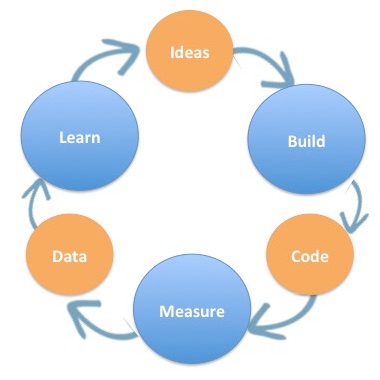
\includegraphics[width=10cm]{figuras/buildmeasurelearn}
\caption{\label{fig:buildmeasurelearn}O ciclo de Build Measure Learn.}
\end{figure}
\begin{itemize}
\item Construir (\emph{Build}): algumas ideias são definidas a partir das hipóteses do produto que precisam ser implementadas no MVP;
\item Medir (\emph{Measure}): implementado o MVP coleta-se os dados de uso, avaliando seu desempenho. Todo o ciclo é baseado na idéia de aprendizado válido para coletar o máximo possível de informação sobre a reação dos usuários.
\item Aprender (\emph{Learn}): a partir da análise dos dados coletados é possível inferir sobre como prosseguir o desenvolvimento e definir novas hipóteses para iniciar um novo ciclo.
\end{itemize}
\par As etapas do ciclo não precisam necessariamente ocorrer em ordem podendo se sobrepor ou mesmo serem unidas dependendo de como for o ciclo de desenvolvimento  \citep{ries:11}.
\par As alterações de software precisam ser feitas de maneira rápida, de modo a testar o mais rápido possível novas ideias. Portanto, é importante que as funcionalidades sejam simples e diretas. O foco é o aprendizado e não desenvolver um software ou um protótipo completo.
\par Para minimizar o risco de que um sistema com problemas seja colocado em produção e acelerar o processo de desenvolvimento, procura-se utilizar ferramentas que auxiliem na integração contínua do software, além da execução de testes automatizados. A utilização desses recursos permite manter um desenvolvimento consistente e confiável sem comprometer o tempo de execução.
\par O que o Construir-Medir-Aprender perde de vista é que novos empreendimentos, tanto \emph{startups} quanto novas iniciativas dentro de empresas já existentes, não começam com ideias mas com hipóteses.
\par O conceito de ``Ideia'' evoca uma visão que imediatamente requer um plano para se frutificar. Em contraste, ``hipótese'' indica um palpite com precedentes que requer experimentação e dados para ser validado ou invalidado. \citep{blankendeavor}
\par Como a construção deve estar alinhada com as hipóteses formuladas e a cada ciclo é necessário sempre testar novas hipóteses, a figura \ref{fig:hypotheses-experiment} representa uma variação do ciclo de Construir-Medir-Aprender, cuja proposta é enfatizar quais hipóteses devem ser testadas.
\begin{figure}[htb]
\centering
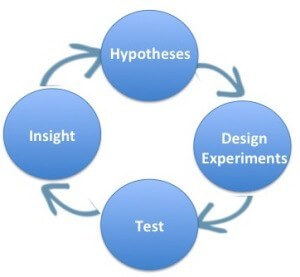
\includegraphics[width=5cm]{figuras/hypotheses-experiment}
\caption{\label{fig:hypotheses-experiment} Uma variação para o ciclo de Construir-Medir-Aprender.}
\end{figure}

\section{Desenvolvimento de Clientes}
\par Steve Blank, em seu livro ``Os 4 passos para a epifania'', explica que o modelo de Desenvolvimento de Clientes não é um substituto para o modelo de Desenvolvimento de Produto e que na verdade ambos devem ser executados em paralelo. No mesmo livro ele define o modelo de Desenvolvimento de Clientes de uma \emph{startup} com a premissa: “Aprender e descobrir quem são os clientes iniciais de uma empresa, e em quais mercados eles estão, requer um processo separado e distinto do Desenvolvimento de Produtos. A soma dessas atividades é o Desenvolvimento de Clientes”. \citep{blank:03}
\par É um processo interativo que parte da premissa de que os fatos estão fora do escritório. Dentro dele só existem opiniões e, portanto, o empreendedor deve buscar o quanto antes validar suas hipóteses fundamentais no mercado.\footnote{Manual da \emph{Startup} Fonte: \url{http://www.manualdastartup.com.br/blog/customer-development-o-processo-para-se-chegar-ao-productmarket-fit/}}.
\par O processo é dividido em 4 passos (figura \ref{fig:customerdevelopment}), sendo que os dois primeiros acontecem antes do ajuste do produto ao mercado, com foco no aprendizado e validação de hipóteses, enquanto os outros dois têm foco no crescimento e otimizações.
\begin{figure}[htb]
\centering
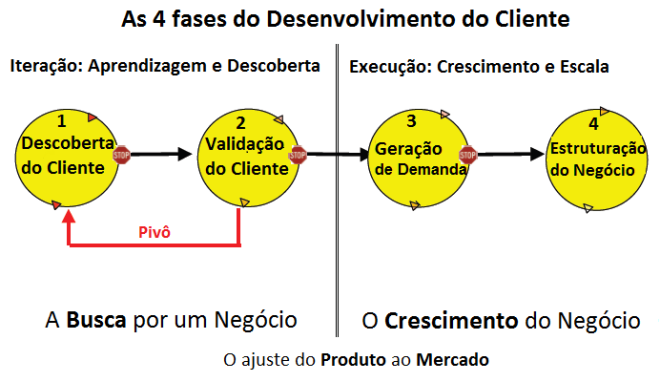
\includegraphics[width=15cm]{figuras/customerdevelopment}
\caption{\label{fig:customerdevelopment}Os 4 passos do ciclo de Customer Development.}
\end{figure}
\par A primeira fase do ciclo é compreendida pelos dois primeiros passos: Descoberta do Cliente e Validação do Cliente. Na Descoberta do Cliente o objetivo é provar que existe um problema a ser solucionado em um mercado grande o suficiente e que o produto supre essa necessidade. Para isso é proposto sempre estar em contato com o cliente, realizando entrevistas de modo a obter um conjunto mínimo de funcionalidades e testá-las em um MVP.
\par Já na etapa de Validação do Cliente o foco é provar que existe uma maneira rentável de se adquirir e manter consumidores. Nessa etapa é necessário descobrir se de fato existem clientes dispostos a pagar pelo produto e se o produto provoca uma mudança na rotina do usuário.
\par A segunda fase, Geração de Demanda e Estruturação do Negócio, é a fase para crescimento do negócio, na qual o foco passa a ser a execução. Nessa fase o foco deixa de ser achar o encaixe de mercado para concentrar-se em escalar o crescimento da empresa.
